\documentclass[border=10pt]{standalone}
\usepackage[svgnames]{xcolor}
\usepackage{amsmath}
\usepackage{pgfplots}
\pgfplotsset{compat=newest}
\usepackage[sfdefault]{FiraSans}
\usepackage{FiraMono}
\renewcommand*\familydefault{\sfdefault}
\begin{document}
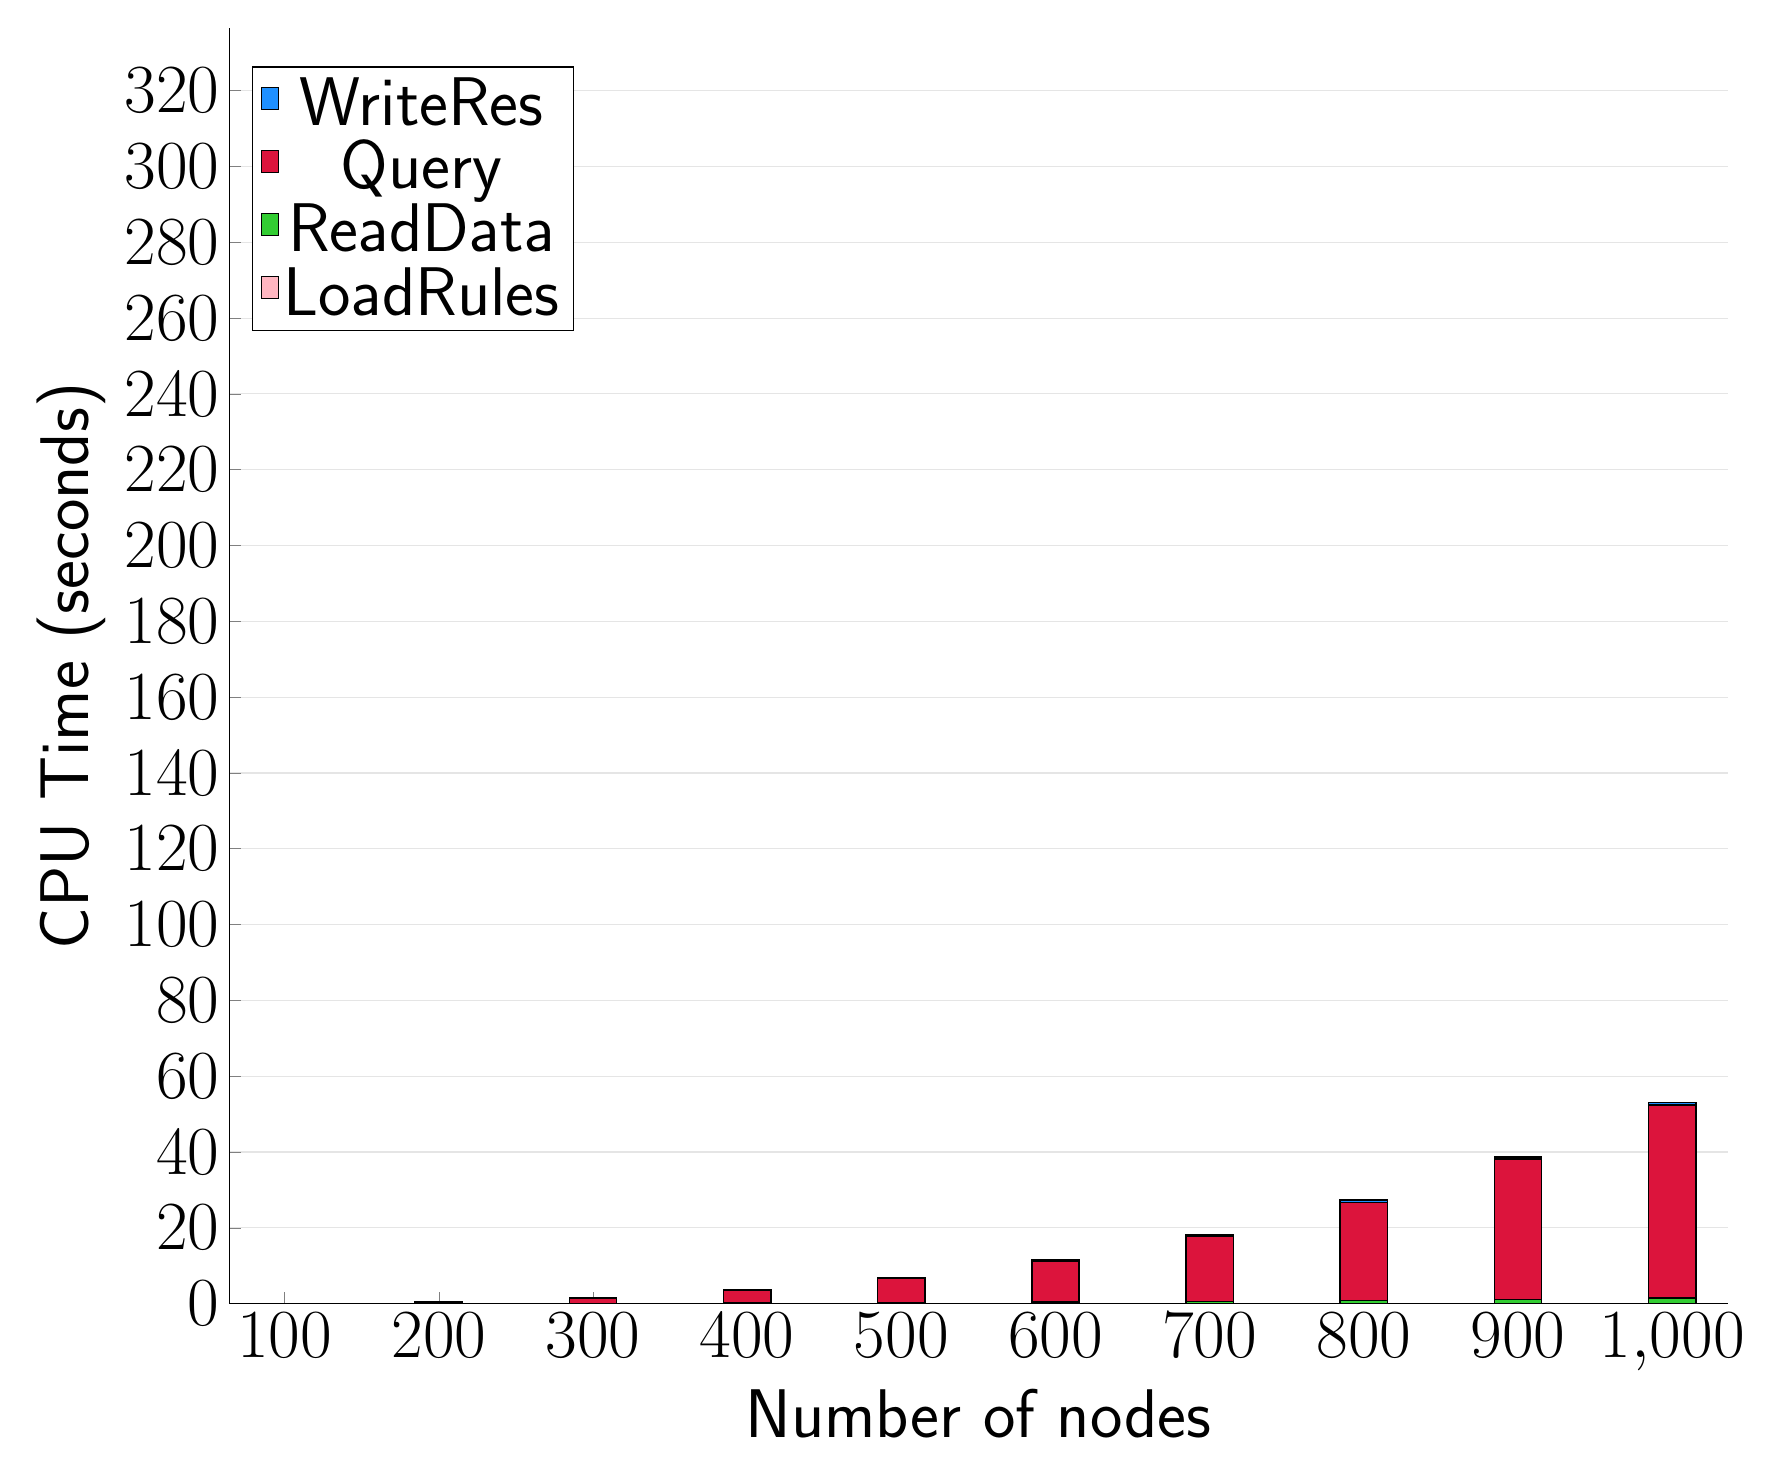
\begin{tikzpicture}
\begin{axis}[
   ybar stacked,
   width=1.7\textwidth,
   bar width=0.6cm,
   ymajorgrids, tick align=inside,
   major grid style={draw=gray!20},
   xtick=data,
   ymin=0, ymax=336.479,
   axis x line*=bottom,
   axis y line*=left,
   enlarge x limits=0.04,
   legend style={
       at={(0.23, 0.97)},
       anchor=north east,
       legend columns=1,
       font=\Huge,
   },
   ylabel={CPU Time (seconds)},
   xlabel={Number of nodes},
   label style={font=\Huge},
   tick label style={font=\Huge},
]
\addlegendimage{fill=DodgerBlue, draw=black, line width=0.2pt}
\addlegendentry{WriteRes}
\addlegendimage{fill=Crimson, draw=black, line width=0.2pt}
\addlegendentry{Query}
\addlegendimage{fill=LimeGreen, draw=black, line width=0.2pt}
\addlegendentry{ReadData}
\addlegendimage{fill=LightPink, draw=black, line width=0.2pt}
\addlegendentry{LoadRules}
\addplot +[fill=LightPink, draw=black, line width=0.55pt] coordinates {
(100, 0.00044340000000000004)
(200, 0.0005123999999999996)
(300, 0.0005789999999999995)
(400, 0.0005461999999999994)
(500, 0.0005488)
(600, 0.0005494000000000001)
(700, 0.0005506000000000004)
(800, 0.0005513999999999999)
(900, 0.0005742000000000005)
(1000, 0.0005633999999999999)
};
\addplot +[fill=LimeGreen, draw=black, line width=0.55pt] coordinates {
(100, 0.007969799999999999)
(200, 0.0334096)
(300, 0.0863796)
(400, 0.1588628)
(500, 0.26448219999999995)
(600, 0.4087526)
(700, 0.595202)
(800, 0.830541)
(900, 1.12971)
(1000, 1.5090992)
};
\addplot +[fill=Crimson, draw=black, line width=0.55pt] coordinates {
(100, 0.049724399999999995)
(200, 0.4057604)
(300, 1.3973334)
(400, 3.2832036)
(500, 6.443149)
(600, 10.820947799999999)
(700, 17.2542082)
(800, 25.908335)
(900, 36.966672599999995)
(1000, 50.868073599999995)
};
\addplot +[fill=DodgerBlue, draw=black, line width=0.55pt] coordinates {
(100, 0.007120600000000002)
(200, 0.0339866)
(300, 0.048069600000000004)
(400, 0.13453820000000008)
(500, 0.19311740000000038)
(600, 0.2464664000000006)
(700, 0.3943799999999996)
(800, 0.5607845999999995)
(900, 0.642662799999998)
(1000, 0.6894846000000001)
};
\end{axis}
\end{tikzpicture}

\end{document}
